\chapter{Marco teórico}
\section{Contenido del marco teórico}
El marco teórico debe explicar, clara y resumidamente, el conocimiento necesario para poder entender el trabajo de título realizado. Puede tocar aspectos matemáticos, informáticos o, por lo general, ambos. Las ecuaciones utilizadas deben ser numeradas y etiquetadas para poder usar referencias cruzadas.

Por ejemplo: 
La Teoría de los Efectos Olvidados fue propuesta por \textcite{kaufmann1988modelos} para identificar efectos indirectos a partir de procesos causa-efecto.

Los efectos olvidados de segundo orden se calculan mediante
\begin{equation}
    CE^{n+1}= CE^{\sum_{i=1}^{n+1}{i}} - CE^{\sum_{i=1}^n{i}}
\end{equation}

donde:
\begin{equation}
    CE^{\sum_{i=1}^{n+1}{i}} = CC \circ CE^{\sum_{i=1}^n{i}} \circ EE
    \label{eq: maxmin_triple}
\end{equation}

y $\circ$ es un operador no lineal y asociativo conocido como convolución maxmin. En términos generales para una matriz cuadrada y reflexiva:
\begin{equation}
    A = [ \mu_{c, \hat{c}}]_{ C \times C} 
\end{equation}

donde la convolución maxmin utilizada en \ref{eq: maxmin_triple} es definida como:

\begin{equation}
    \mu_{c,\hat{c}}^{1+2} = max_{c, \hat{c} = 1,..., C}\{ min_{k = 1,...,C}\{\mu_{c,k}, \mu_{k,\hat{c}} \} \}
    \label{eq: maxmin}
\end{equation}

y los efectos de segundo orden se obtienen de:
\begin{equation}
    \mu_{c,\hat{c}}^{2} = \mu_{c,\hat{c}}^{1+2} - \mu_{c, \hat{c}}
\end{equation}

\section{Figuras\label{Sec: Figuras}}
Las figuras deben ser generadas en PDF, incluidas en el documento y referenciadas usando referencias cruzadas. Por ejemplo:

La Figura \ref{figure: 1d_triangle} muestra un ejemplo simple de efectos olvidados o las relaciones indirectas entre dos nodos de una red. Dado tres nodos $A$, $B$, $C$, de un grafo, y el peso de cada arista $\mu_{a,b}$, $\mu_{a,c}$ y $\mu_{b,c}$ $\in [0\,,\,1]$ , si $min(\mu_{a,b}, \mu_{b,c}) - \mu_{a,c} > 0.5$ es posible decir que la incidencia indirecta $A \rightarrow C$ por medio de $B$ es mas fuerte que la incidencia directa $A \rightarrow C$.
\begin{figure}[H]
  \centering
  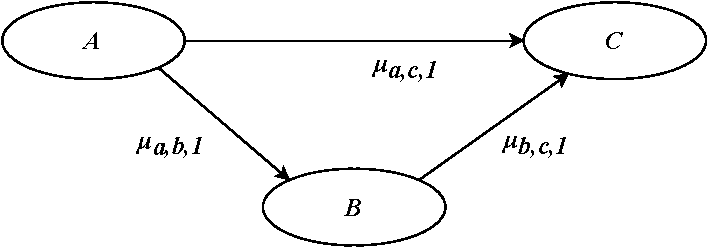
\includegraphics[width=\textwidth]{files/1d.pdf}
  \caption{Ejemplo de relaciones directas e indirectas.}
  \label{figure: 1d_triangle}
\end{figure}

\section{Refencia a secciones anteriores}
Igualmente, cualquier referencia a secciones anteriores debe ser realizada usando referencias cruzadas. Por ejemplo:

Dado que primero necesitaremos definir algunos conceptos, el algoritmo que se utilizará para el cálculo de los efectos indirectos se presentará en la Sección \ref{Sec: Figuras}. 

\section{Cuadros}

Los cuadros deben ser diseñadas de tal manera que se usen únicamente líneas horizontales, dejando las verticales para excepciones muy limitadas. Deben ser referenciadas usando referencias cruzadas. Por ejemplo:

Para el experto $i$, $\mu_{c,\hat{e},i}$ es el grado de verdad entre $[0\,,\,1]$ del enunciado ``$c$ tiene una incidencia sobre $e$'' (equivalente para las otros dos matrices). Las matrices $CC_i$ y $EE_i$ son reflexivas, es decir, son cuadradas y de diagonal igual a 1, pero no necesariamente simétricas. Se debe definir un punto $\varepsilon$ que establece el grado de verdad mínimo de incertidumbre de la afirmación ``$c$ tiene una incidencia sobre $e$''. En el Cuadro \ref{tab:Tabla-de-Verdad} se puede apreciar la tabla endecadaria habitualmente usada en entrevistas de expertos para identificar este grado de verdad \parencite{kaufmann1993tecnicas}, en donde $\varepsilon=0,5$. No obstante, el paquete puede trabajar con escalas continuas en el intervalo $[0\,,\,1]$, permitiendo un granularidad más fina en la evaluación de los grados de verdad de las relaciones y valores de $\varepsilon$ particulares para el caso estudiado.. 

\begin{table}
\centering
\begin{tabular}{|l|l|}
\hline
\textbf{Grados de Verdad} & \textbf{Evaluación}     \\ \hline
0                         & Falso                   \\ \hline
0,1                       & Prácticamente falso     \\ \hline
0,2                       & Casi falso              \\ \hline
0,3                       & Bastante falso          \\ \hline
0,4                       & Más falso que verdadero \\ \hline
0,5                       & Ni verdadero ni falso   \\ \hline
0,6                       & Más verdadero que falso \\ \hline
0,7                       & Casi verdadero          \\ \hline
0,8                       & Bastante verdadero      \\ \hline
0,9                       & Prácticamente verdadero \\ \hline
1                         & Verdadero               \\ \hline
\end{tabular}
\caption{Tabla endecadaria de grados de verdad.}
\label{tab:Tabla-de-Verdad}
\end{table}

\section{Algoritmos}
Los algoritmos deben ser presentados en un pseudo-código muy resumido, prefiriendo la notación matemática en su lugar. Deben ser creados usando las clases \texttt{algorithm} y \texttt{algorithmic}, así como ser referenciados usando referencias cruzadas.

La matriz conjugada de orden $n$, $CE^{\sum_{i=1}^{n}{i}}$, contiene todos los efectos directos y olvidados que se han encontrado hasta ese momento. Para encontrar $CE^{n+1}$, debe sustraerse de la matriz conjugada de orden $n+1$ la matriz conjugada de orden $n$. Se actualiza, tomando como referencia $\varepsilon$, la lista de efectos de orden $n+1$ según el Algoritmo \ref{FE.recursive}. $CE^{n+1}$ es una matriz de ceros únicamente cuando ya no existen efectos olvidados de grado $n+1$ o superior, por lo que el algoritmo se detiene y retorna los efectos olvidados identificados en la lista $edges$.

\begin{algorithm}
\begin{algorithmic}[1]
\caption{\textsc{FE.recursive}}
\label{FE.recursive}
\Variables
 \State $n$
 \State $edges$
\EndVariables
\Procedure{FE.recursive}{$CC_{i}, CE^{\sum_{i=1}^n{i}}, EE_{i}, \varepsilon \in [0,1], maxOrder \geq 2, CE^{n}$}
\State $n \Leftarrow n + 1$
%\State $edges \Leftarrow$ elements of $CE^n> \varepsilon$
\If{ $\left| \textbf{ elements of } CE^n > \varepsilon \right| = 0 \textbf{ or } n \geq maxOrder + 1$}
    \State \textbf{return} $edges$ 
\EndIf
    %\State $CE^{\sum_{i=1}^{n+1}{i}} \Leftarrow$ \Call{maxmin}{\Call{maxmin}{$CC_{i},CE^{\sum_{i=1}^n{i}}$}$,EE_{i}$}
    \State $CE^{\sum_{i=1}^{n+1}{i}} \Leftarrow$ \textsc{maxmin}(\textsc{maxmin}($CC_{i},CE^{\sum_{i=1}^n{i}}$)$,EE_{i}$)
    \State $CE^{n+1} \Leftarrow CE^{\sum_{i=1}^{n+1}{i}} - CE^{\sum_{i=1}^n{i}}$
    \State \Call{FE.recursive}{$CC_{i}, CE^{\sum_{i=1}^{n+1}{i}}, EE_{i}, \varepsilon, maxOrder,CE^{n+1}$}
    %\State \textbf{Update} $edges$  \textbf{with elements of}   $CE^{n+1}> \varepsilon$
    %\State \textbf{Update} $FE.list$ \textbf{with} $\Call{Seek.Paths}{edges, CC_{i}, CE^{\sum_{i=1}^{n}{i}}, EE_{i}, CE^{n+1}}$
    \State $n \Leftarrow n - 1$
    
    \State \textbf{Update} $edges \textbf{ with elements of } CE^{n+1} \geq \varepsilon$
    
    \State \textbf{Update} $edges$ \textbf{with} $\Call{Seek.Paths}{edges, CC_{i}, CE^{\sum_{i=1}^{n+1}{i}}, EE_{i}, CE^{n+1}}$

\State \textbf{return} $edges$
\EndProcedure
\end{algorithmic}
\end{algorithm}

